\item \points{1} {\bf Data Processing for Few-Shot Classification}

Before training any models, you must write code to sample batches for training. Fill in the \texttt{\_sample} function in the \texttt{DataGenerator} class. The class already has variables defined for batch size \texttt{batch\_size} ($B$), number of classes \texttt{num\_classes} ($N$), and number of samples per class \texttt{num\_samples\_per\_class} ($K+1$). Your code should:
\begin{enumerate}
    \item Sample $N$ different characters from either the specified train, test, or validation folder.
    \item Load $K+1$ images per character and collect the associated labels, using $K$ images per class for the support set and 1 image per class for the query set.
    \item Format the data and return two tensors, one of flattened images with shape [$K+1, N, 784$] and one of one-hot labels [$K+1, N, N$].
\end{enumerate}  

\begin{figure}
    \centering
    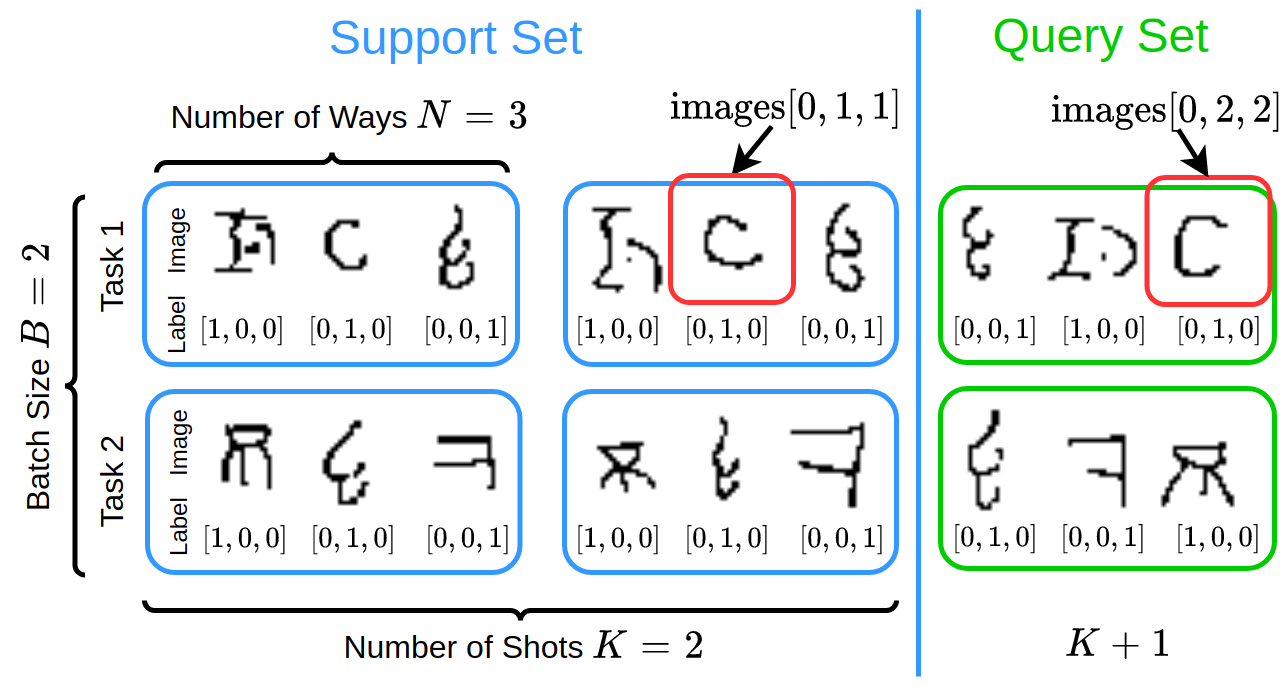
\includegraphics[width = 0.75\textwidth]{./figures/ps2_batch}
    \vspace{-0.3cm}
    \caption{\small Example data batch from the Data Generator. The first $K$ sets of images form the support set and are passed in the \emph{same order}. The final set of images forms the query set and must be shuffled.}
    \label{fig:batch}
\end{figure}
Note that your code only needs to return one single (image, label) tuple. We batch the inputs using an instance of torch.utils.data.DataLoader, and the final shape input images is [$B, K+1, N, 784$], and that of the input labels is [$B, K+1, N, N$], where B is the batch size.

Figure \ref{fig:batch} illustrates the data organization. In this example, we have: (1) images from $N=3$ different classes; (2) we are provided $K=2$ sets of labeled images in the support set and (3) our batch consists of only two tasks, i.e. $B=2$. 
\begin{enumerate}
    \item We will sample both the support and query sets as a single batch, hence one batch element should obtain image and label tensors of shapes $[K+1, N, 784]$  and $[K+1, N, N]$ respectively. In the example of Fig. \ref{fig:batch}, \texttt{images[0, 1, 1]} would be the image of the letter "C" in the support set with corresponding class label $[0, 1, 0]$ and \texttt{images[0, 2, 2]} would be the the letter "C" in the query set (with the same label).

    \item We must shuffle the order of examples in the \textbf{query set}, as otherwise the network can learn to output the same sequence of classes and achieve 100\% accuracy, without actually learning to recognize the images. If you get 100\% accuracy, you likely did not shuffle the query data correctly. In principle, you should be able to shuffle the order of data in the support set as well; however, this makes the model optimization much harder. \textbf{You should feed the support set examples in the same, fixed order}. In the example above, the support set examples are always in the same order.

\end{enumerate}

\noindent We provide helper functions to (1) take a list of folders and provide paths to image files/labels, and (2) to take an image file path and return a flattened numpy matrix. The functions \texttt{np.random.shuffle} and \texttt{np.eye} will also be helpful. \textbf{Be careful about output shapes and data types!}

\clearpage

